\section{Experimental setups}\label{sec:setup}

\subsection{Key components}
\paragraph{Scintillation detector}
detects ionizing radiation in general. Here only gamma radiation is relevant. The purpose of scintillator is to lower photon energy via photoelectric effect, Compton scattering, and pair production~\cite{wermes}. It is then connected to photomultiplier tube (PMT) to generate signals.
\begin{figure}[ht]
   \centering
   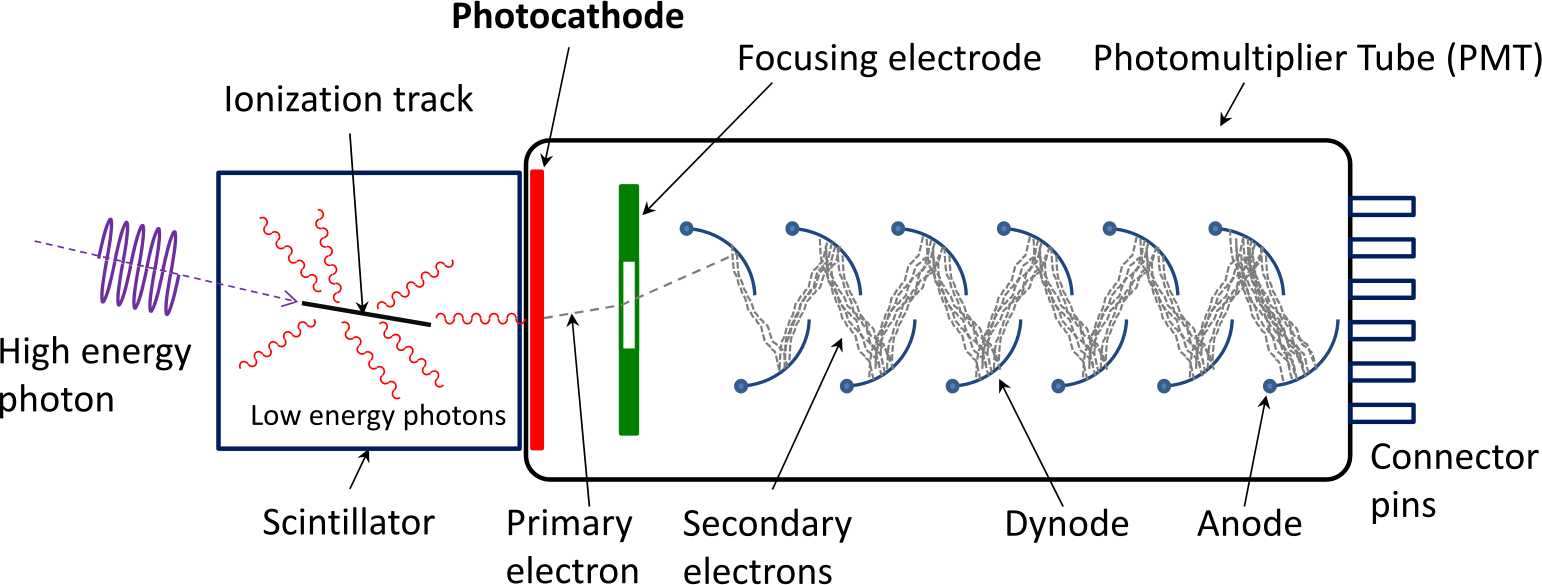
\includegraphics[width=0.7\linewidth]{Scintillator.png}
   \caption{Scintillator with PMT~\cite{wikiScin}}%
\end{figure}


\paragraph{Fast-slow coincidence} is the technique to measure the ionizing radiation separately. The "slow" part will determine the energy of incoming radiation. And the "fast" part is used to measure the time as precisely as possible, since the photomultiplier will be brought to saturation and the height of the pulse is not proportional to radiation energy any more~\cite{IACI1968103}. 

\paragraph{SCA} stands for single channel analyzer. Basically it is advanced version of simple discriminator, as one can set both upper-level (ULD) and lower-level discriminator (LLD) for SCA. It reads the input pulse and check whether it is within the preset limits or not. If it is, SCA will produce a uniform digital signal.
When applied to PMT, the height of pulse corresponds to energy of radiation. If SCA is built in after PMT, we are essentially picking out photons within the SCA window. Thus the name~\cite{SCAmanual}.

\begin{figure}[ht]
	\centering
	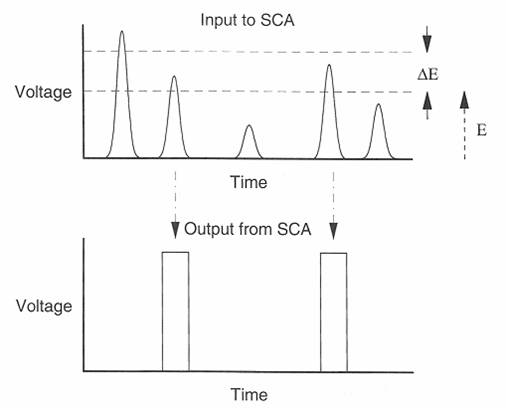
\includegraphics[width=0.5\linewidth]{sca-binning.jpg}
	\caption{Single Channel Analyzer~\cite{wikiScin}}%
\end{figure}


% Simple discriminator outputs logic signal right after input goes higher than threshold. Since SCA also needs to check the ULD, it will produce output after maximal amplitude. There are two modes: non-timing and timing SCA. Non-timing SCA generates output right after the input comes back to the LLD, i.e.~after its peak. It will create the so-called "time walk" meaning that logic output will differ in time, even thought the inputs are simultaneous but of different height. Timing SCA, on the other hand, outputs logic signal as soon as the input hits its maximum~\cite{SCAmanual}.

%TODO: too much explanation, need to cut before hand in!

\paragraph{CFD} stands for constant fraction discriminator. As its name suggests, it gets triggered at some preset fraction of maximal amplitude, in order to reduce "walk". In simplest form, CFD works by splitting input signals, inverting one of them, and adding delay to the other. In the end, by combining these two together, we get logic signal with minimal walk~\cite{CFDmanual}.


%TODO: actually three parts, relating to comparator. Can adjust delay to cope with different rise time

% \paragraph{TAC} stands for time-to-amplitude converter, which outputs pulse with amplitude proportional to time difference between start and end signals.

% \paragraph{Time resolution} of fast coincidence unit is $< \SI{100}{\nano\s}$ on any single input and $< \SI{1}{\mu\s}$ on the coincidence output~\cite{fastmanual}.

\paragraph{Expected Spectrum} of ${}^{60} \text{Co}$ would predominantly consists of $\SI{0.31}{\mega\eV}$ $\beta$-line and \SI{1.1732}{\mega\eV}, \SI{1.3325}{\mega\eV} $\gamma$-line~\cite{firestone}. Its $\gamma$-spectrum can be found in~\ref{fig:CoSpec}, where one can see two clear peaks corresponding to the $\gamma$-radiations and some background because of various effects, like pair production (higher $E$), Compton scattering (mid $E$), and photoelectric effect (low $E$)~\cite{wermes}.

\begin{figure}[ht]
   \centering
   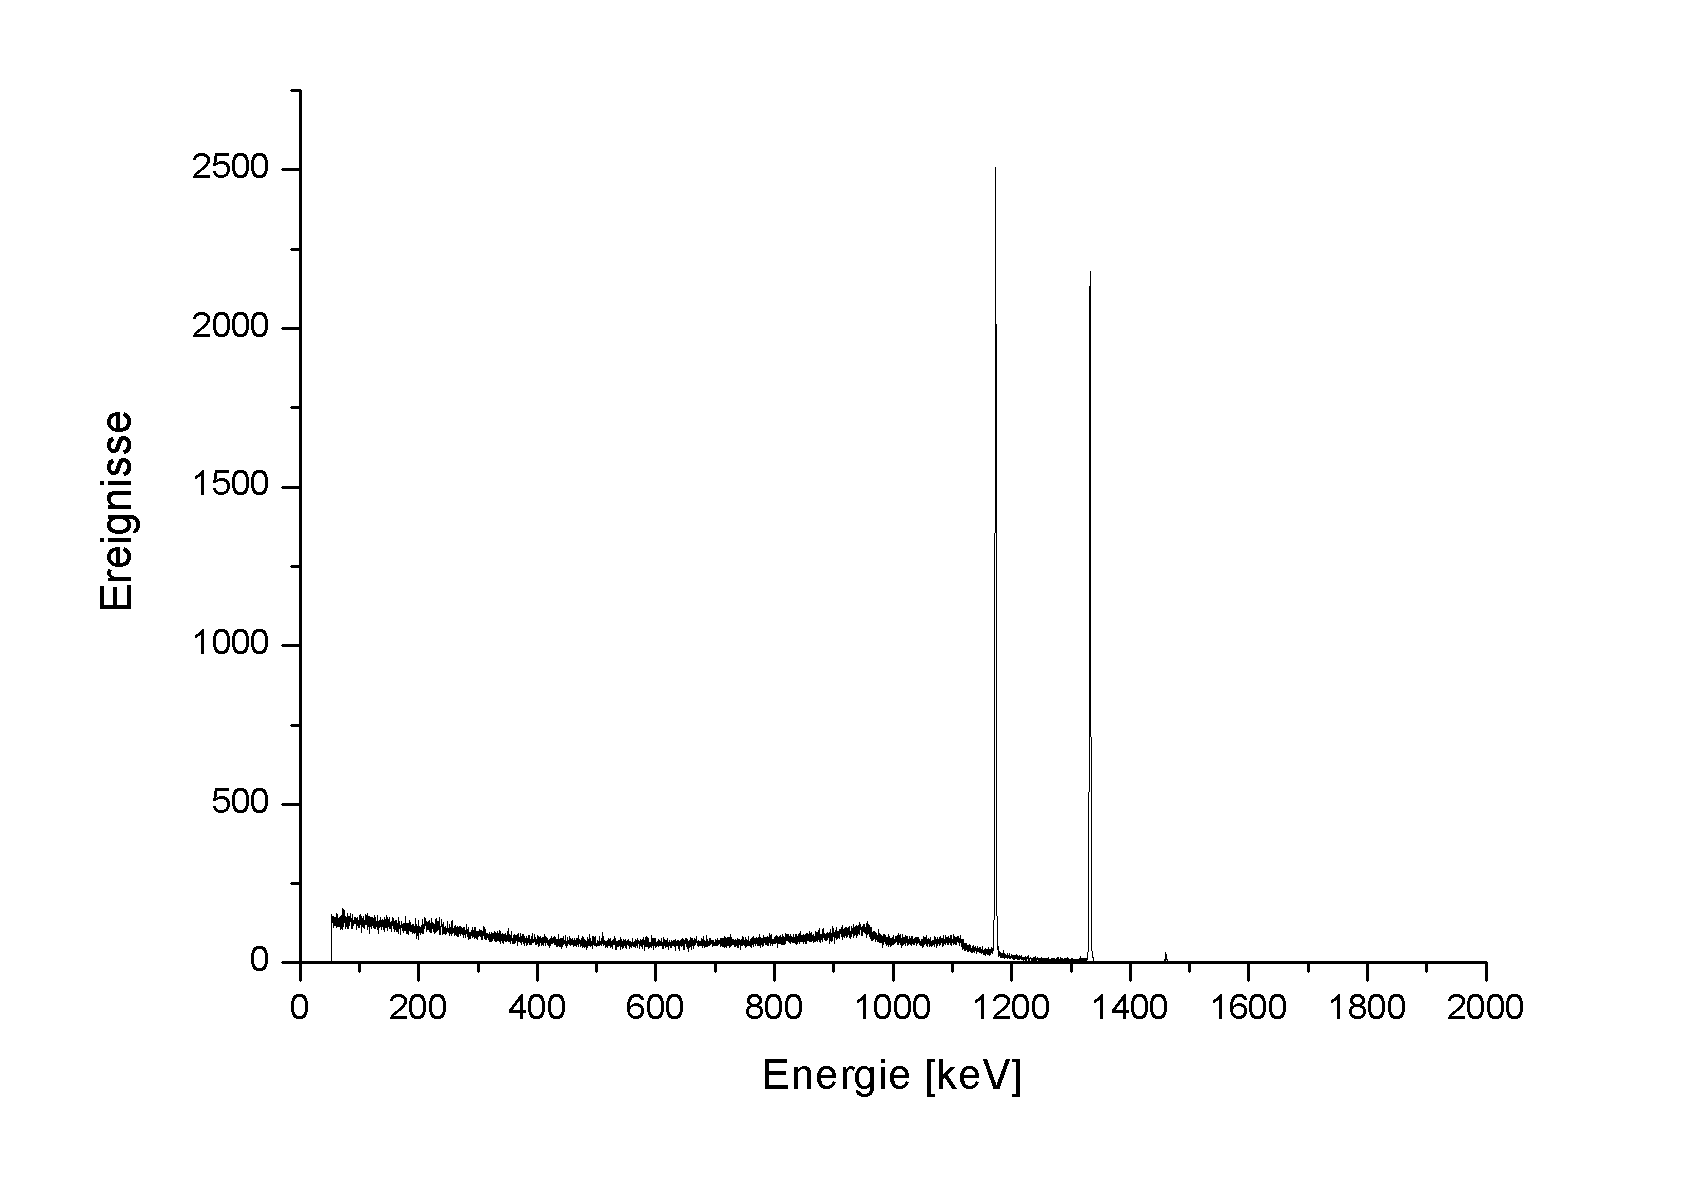
\includegraphics[width=0.6\linewidth]{60Co_gamma_spectrum_energy.png}
   \caption{${}^{60}\text{Co}$ $\gamma$-specturm~\cite{CoSpec}}%
   \label{fig:CoSpec}
\end{figure}

\section{Task for preparation}\label{sec:task}
\subsection{Which distances to pick?}
Obviously, the count (rate) should be proportional to the solid angle ignoring the anisotropy of radiation. This assumption should not bring too much influence to the results, as long as the size of detection is accounted for in final analysis as (systematic) error. In~\cite{siegbahn}, true count rate is given by
\begin{equation}
   N^t_i (\theta) = M p_i \Omega_i \epsilon_i
\end{equation}
with $M$ the number of nuclear integrations per uni time, $p_i$ the probability that this integration is selected, $\Omega_i$ is solid angle in unit $4\pi$, and $\epsilon_i$ the detector efficiency. According to formula of solid angle, it means that
\begin{equation}
   N^t_i (\theta) \propto \frac{1}{r_i^2}
\end{equation}

Follow the same principle, true number of coincidence can be written as~\cite{siegbahn}
\begin{equation}
   C^t(\theta) = M p_1 p_2 \Omega_1 \epsilon_1 \Omega_2 \epsilon_2 \epsilon_c K(\theta)
\end{equation}
where $\epsilon_c$ is the efficiency of coincidence unit and $K(\theta)$ is the directional correlation function. $K(\theta)$ is basically the "measured" version of $W(\theta)$, i.e.~what we have in the real world. 
The coincidence rate is then $C^t(\theta)/ N_1^t(\theta)$ thus 
\begin{equation}
   \frac{C^t(\theta)}{N_1^t(\theta)} \propto \frac{1}{r_2^2}
\end{equation}

The angular "asymmetry" is represented as the coefficients $A_{kk}$. With correction factor, we write
\begin{equation}
   A_{kk} = \frac{A_{kk}^\text{exp}}{Q_{kk}}
\end{equation}
And it can be calculated by~\cite{siegbahn}
\begin{align}
   Q_{kk} &= Q_k(1) Q_k(2) \\
   Q_k(i) &= \frac{J_k(i)}{J_0(i)} \\
   J_k(i) &= \int_0^{\pi/2} \epsilon_i (E,\alpha) P_k (\cos\alpha) \sin \alpha \dd{\alpha} \\
   \epsilon(E,\alpha) &= 1 - \exp{- \tau (E) X(\alpha)}
\end{align}
with $\tau (E)$ the total absorption coefficient and $X(\alpha)$ the distance traversed in the crystal.

The correction factor will certainly affect the error of angular correlation function, multiplicatively to be specific.

According to table in~\cite{siegbahn}, $h=\SI{10}{\cm}$ would provide the most precise measurement, since the $Q_i$'s are closer to $1$. So in the actual experiment, one can try to measure the event rate in a short time period. Then the distance should be so chosen that enough data will be taken in the given time but still have maximal precision.

\subsection{Which angles to pick?}
The angular correlation function is given in the form of~\cite{descr}
\begin{equation}
   f(\theta) = A(1 + B \cos^2\theta + C \cos^4 \theta)
   \label{math:fTheta}
\end{equation}
It can be rewritten with $\alpha= B + C$ and $\beta = B-C$,
\begin{equation}
   f(\theta) = A \left( 1 + \frac{\alpha + \beta}{ 2} \cos^2\theta + \frac{\alpha-\beta}{2} \cos^4 \theta \right)
\end{equation}

Predicted values for $A_{22}$ and $A_{44}$ without mixing are given in~\cite{siegbahn}. Then the predicted correlation function is
\begin{align}
   \begin{split}
   W(\theta) &= 1 - \frac{A_{22}}{2} + \frac{3}{8} A_{44} + \left( \frac{3}{2} A_{22} - \frac{15}{4} A_{44} \right) \cos^2 \theta + \frac{35}{8} A_{44} \cos^4 \theta \\
   &= 0.952412 + 0.118875 \cos^2 \theta + 0.039813 \cos^4 \theta
   \end{split}\label{math:pred}
\end{align}
Need to "scale" it, so that $0.9524$ gets absorbed in $A$. Then we have
\begin{equation*}
   B=0.124815, C=0.041802
\end{equation*}

Plot correlation with these two coefficients with slight variation, we have figure.~\ref{fig:alpha-beta}
\begin{figure}[ht]
   \centering
   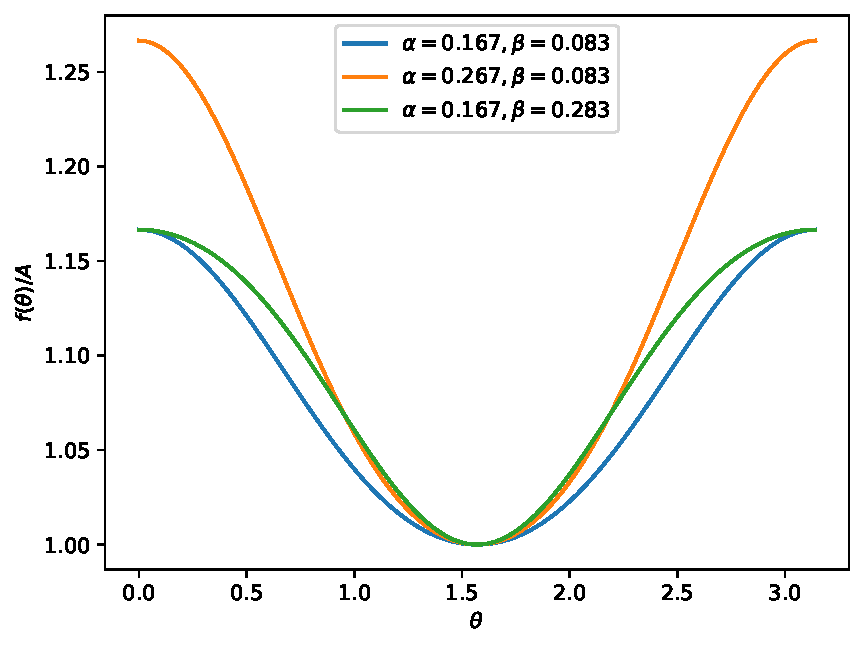
\includegraphics[width=0.6\linewidth]{alpha-beta.pdf}
   \caption{Correlation with different $\alpha$ and $\beta$}%
   \label{fig:alpha-beta}
\end{figure}
From it, it is clear that to determine $\alpha$, we need in principle only one point ($\theta=0$ or $\theta=\pi$). But determination of $\beta$  requires small increments in angle between $0$ and $\pi/2$.

\subsection{How to correct for de-adjustment?}
In actual setup, the source might not lie perfectly in the center of circle of detectors. It will certainly cause a distortion in data, since extra "angular correlation" will be introduced. Depending on in which direction the source is off from the center of circle, the angular correlation could have an obvious asymmetry or just simply gets stretched out. To correct this, count rates of two detectors needs to be recorded. Coincidence rate should be normalized against these count rates.
